\graphicspath{{./images/}}

\chapter{Bausteinsicht}

\section{Beschreibung}

Die Architektur für die Applikation wird mittels vier Schichten realisiert. Die Präsentationsschicht ist auf dem WebServer während die anderen drei sich auf dem AppServer befinden. Die einzelnen Komponenten wurden gruppiert um die Übersicht zu wahren. Auf der nächsttieferen Ebene sind diese Komponenten detailierter aufgeführt.

\newgeometry{left=2.5cm, right=2.5cm, bottom=2.5cm, top=2.5cm}
\begin{landscape}
\section{Ebene 1}

\begin{center}
	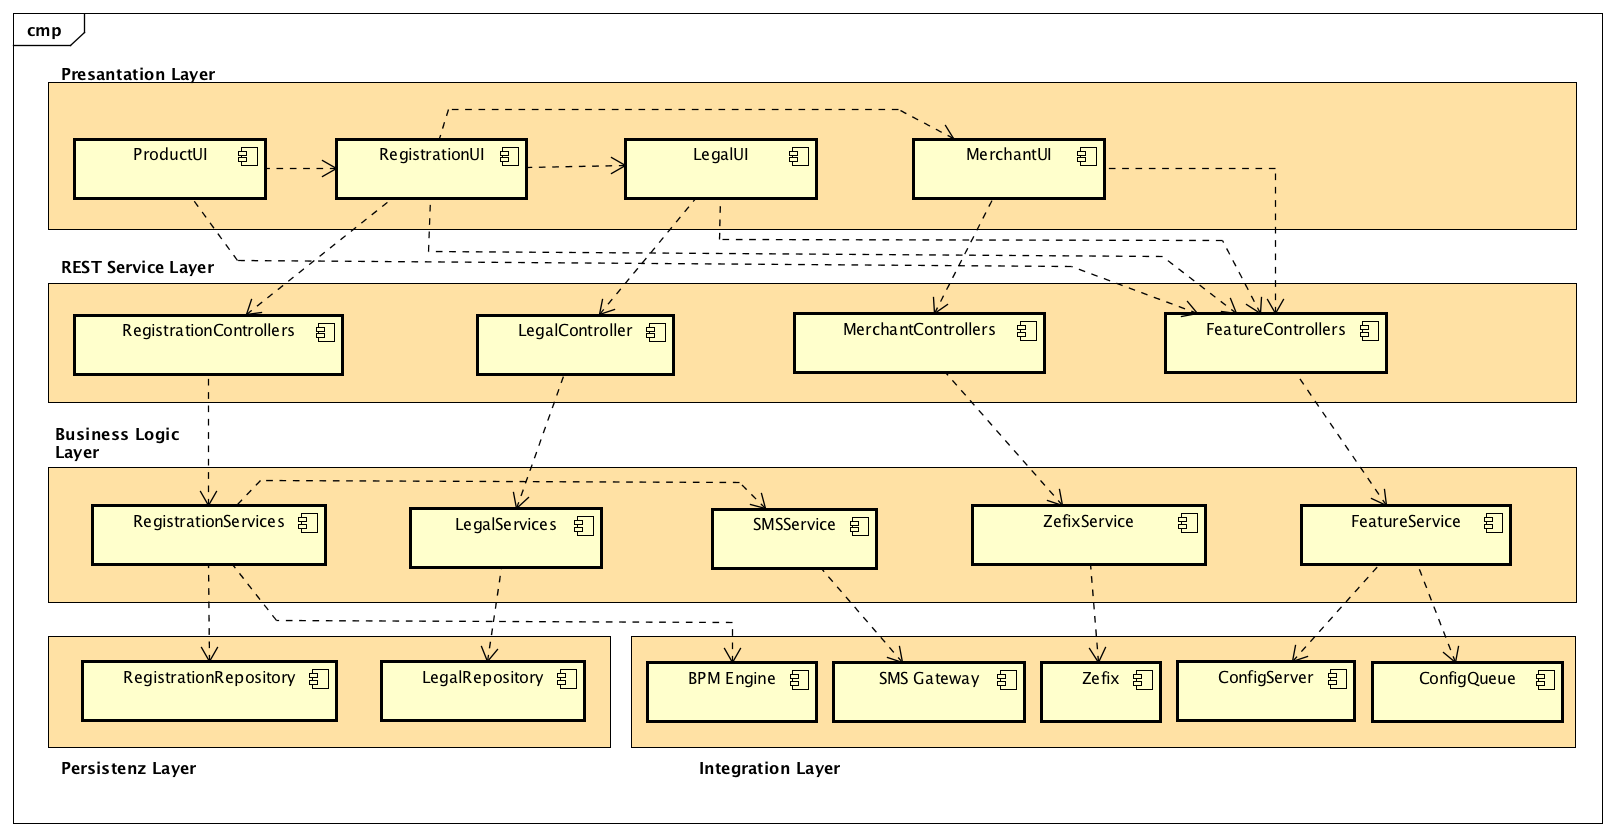
\includegraphics[scale=0.6]{ComponentLevel1.png}
\end{center}

\end{landscape}
\restoregeometry

\begin{table}[H]
	\centering
	\caption{Presentation Layer}
	\begin{tabular}{ | p{4cm} | p{12cm} | }
		\toprule
		{\textbf{Komponente}} & {\textbf{Beschreibung}} \\
		\midrule
		ProductUI &  .. \\ \hline
		RegistrationUI &  .. \\ \hline
		LegalUI &  .. \\ \hline
		MerchantUI &  .. \\
		\bottomrule
	\end{tabular}
\end{table}

\begin{table}[H]
	\centering
	\caption{REST Service Layer}
	\begin{tabular}{ | p{4cm} | p{12cm} | }
		\toprule
		{\textbf{Komponente}} & {\textbf{Beschreibung}} \\
		\midrule
		RegistrationController &  .. \\ \hline
		LegalController &  .. \\ \hline
		VerificationController &  .. \\ \hline
		FeatureController &  .. \\
		\bottomrule
	\end{tabular}
\end{table}

\begin{table}[H]
	\centering
	\caption{Business Logic Layer}
	\begin{tabular}{ | p{4cm} | p{12cm} | }
		\toprule
		{\textbf{Komponente}} & {\textbf{Beschreibung}} \\
		\midrule
		RegistrationService &  .. \\ \hline
		LegalService &  .. \\ \hline
		ZefixService &  .. \\ \hline
		PEPCheckService &  .. \\
		\bottomrule
	\end{tabular}
\end{table}

\begin{table}[H]
	\centering
	\caption{Persistenz Layer}
	\begin{tabular}{ | p{4cm} | p{12cm} | }
		\toprule
		{\textbf{Komponente}} & {\textbf{Beschreibung}} \\
		\midrule
		RegistrationRepository &  .. \\ \hline
		LegalRepository &  .. \\
		\bottomrule
	\end{tabular}
\end{table}

\section{Ebene 2}

\section{Ebene 3}